%% IEEE ICT-PEP 2026 — Transformer LoL Solar Paper
%% Author: Fakhri Hakim, PT PLN (Persero)
%% Compile: pdflatex main && bibtex main && pdflatex main && pdflatex main

\documentclass[conference]{IEEEtran}
\IEEEoverridecommandlockouts

\usepackage{cite}
\usepackage{amsmath,amssymb,amsfonts}
\usepackage{algorithmic}
\usepackage{graphicx}
\usepackage{textcomp}
\usepackage{xcolor}
\usepackage{booktabs}
\usepackage{url}

\def\BibTeX{{\rm B\kern-.05em{\sc i\kern-.025em b}\kern-.08em
    T\kern-.1667em\lower.7ex\hbox{E}\kern-.125emX}}

\begin{document}

\title{Transformer Loss-of-Life Acceleration under High Rooftop-PV Penetration on Indonesian 150/20~kV Substations: A Hybrid IEEE C57.91 + XGBoost Simulation}

\author{\IEEEauthorblockN{Fakhri Hakim}
\IEEEauthorblockA{\textit{PT PLN (Persero)} \\
Jakarta, Indonesia \\
fakhrihakim20@gmail.com}
}

\maketitle

\begin{abstract}
Power transformers at tropical 150/20~kV substations face accelerated insulation aging from the combined pressures of rooftop-PV reverse power flow, ambient warming, and load growth. Quantifying these interacting stresses requires Monte-Carlo (MC) sweeps over thousands of scenario--seed combinations, which is computationally prohibitive with the IEEE~C57.91-2011 differential thermal model alone. This paper presents a reproducible hybrid framework that couples the C57.91 ordinary-differential-equation (ODE) thermal solver with an XGBoost surrogate trained on 200 ODE trajectories, validated to 0.230~$^\circ$C root-mean-square error (RMSE) and $R^2 = 0.9998$. A two-bus PyPSA network model of the 60~MVA ONAF transformer at GI~Jember (East Java, Indonesia) provides scenario-selectable battery dispatch in either threshold-rule or HiGHS linear-program (LP) form. Across 41~scenarios $\times$ 1\,000 MC runs (53~min wall-clock, $474\times$ single-scenario speedup at 1\,000 runs), rooftop-PV monotonically reduces annual loss-of-life (LoL) by up to 19\,\% at 75\,\% penetration; a +1~$^\circ$C ambient and +4.5\,\%/yr load growth raise LoL by 43\,\%, and 75\,\% PV cannot fully restore today's no-PV baseline under projected 2030 conditions. Adding 30\,\% EV fleet penetration raises LoL by 42\,\% relative to the same PV level --- erasing the solar benefit entirely and pushing LoL 18\,\% above the no-PV baseline. A 5~MWh / 2.0~MW battery yields only a further $-1.5\,\%$ LoL reduction, and PyPSA economic-dispatch LP is +1.2\,\% \emph{worse} than the threshold rule --- economic optimisation is not aging-optimal.
\end{abstract}

\begin{IEEEkeywords}
Transformer aging, IEEE C57.91, loss-of-life, rooftop photovoltaic, EV charging, XGBoost surrogate, PyPSA, Monte Carlo, Indonesia, Jember.
\end{IEEEkeywords}

\section{Introduction}
\label{sec:intro}

Indonesia's national utility, PT~PLN (Persero), operates more than 5\,000 power transformers across the Java--Bali 150/20~kV network. The recently revised RUPTL (electricity supply business plan) targets aggressive renewable deployment to support the country's 2060 net-zero pathway~\cite{pln2025ruptl,iea2024indonesia,iesr2024outlook,adb2020indonesia}. While rooftop PV is generally welcomed at the bulk-system level, its cumulative effect on individual substation power transformers is more nuanced: the daytime midday load reduction lowers winding temperatures, but high penetrations can introduce reverse power flow, harmonic exposure, and changed thermal duty cycles.

Transformer insulation aging is governed by an Arrhenius reaction whose rate doubles for every 6~$^\circ$C above 110~$^\circ$C hot-spot temperature ($\theta_{HS}$)~\cite{ieee_c5791_2011}. A single severe thermal excursion can consume months of equivalent service life, and the consequence of premature failure is severe: a replacement 60~MVA power transformer costs roughly USD~800\,000, with 6--12 month logistic lead times in remote regions. Predicting how rooftop PV will alter the lifetime of individual substation assets therefore has direct economic and operational value.

Existing studies of PV impact on transformer aging~\cite{pezeshki2014pv,gaikwad2025evpv,majeed2022reverse} typically run a small number of deterministic scenarios using the C57.91 ODE solver, limiting the resolution of joint sensitivity to climate warming, load growth, and dispatch strategy. Recent work~\cite{chen2025climate} has begun coupling random-forest surrogates with global climate models to enable larger MC sweeps. We extend this direction by combining a fast XGBoost surrogate~\cite{chen2016xgboost} with a PyPSA~\cite{brown2018pypsa} two-bus network model that supports both heuristic and linear-program (LP) battery dispatch. The contributions of this paper are:

\begin{itemize}
    \item A hybrid IEEE~C57.91 + XGBoost surrogate framework that reproduces $\theta_{HS}$ within 0.230~$^\circ$C RMSE while delivering up to $474\times$ wall-clock speedup over the ODE baseline (at 1\,000 runs per scenario).
    \item A two-bus PyPSA model of the GI~Jember 60~MVA ONAF transformer with scenario-selectable battery dispatch (threshold rule or HiGHS LP), enabling direct comparison of dispatch strategies on aging.
    \item A 41-scenario, 1\,000-run Monte-Carlo sensitivity analysis quantifying the joint effect of PV penetration, climate warming, load growth, EV charging, and battery storage on annual loss-of-life.
    \item A reproducible open-source release with a GI~Jember case-study calibration and explicit BMKG, PLN, and ERA5/atlite data hooks; when those files are unavailable, documented synthesis fallbacks preserve the same code path for peer replication.
\end{itemize}

\section{Methodology}
\label{sec:method}

\subsection{IEEE C57.91 Thermal Model and Harmonic Loss Uplift}
\label{sec:method-thermal}
The top-oil temperature rise $\Delta\theta_{TO}$ and hot-spot rise $\Delta\theta_{HS}$ above the oil are governed by the differential-equation form of the 2011 edition of IEEE~Std~C57.91~\cite{ieee_c5791_2011,iec_60076_7_2018,lesieutre1997topoil}:
\begin{align}
\tau_{TO}\frac{d\Delta\theta_{TO}}{dt} &= \Delta\theta_{TO,U} - \Delta\theta_{TO}, \label{eq:to}\\
\tau_{W}\frac{d\Delta\theta_{HS}}{dt} &= \Delta\theta_{HS,U} - \Delta\theta_{HS}, \label{eq:hs}
\end{align}
where the ultimate values for loading factor $K(t) = S(t)/S_{rated}$ are
\begin{align}
\Delta\theta_{TO,U} &= \Delta\theta_{TO,R}\!\left[\frac{K^{2}\!R + 1}{R + 1}\right]^{\!n}\!, \\
\Delta\theta_{HS,U} &= \Delta\theta_{HS,R}\,K^{2m}.
\end{align}
The hot-spot temperature is then $\theta_{HS}(t) = \theta_{a}(t) + \Delta\theta_{TO}(t) + \Delta\theta_{HS}(t)$. We solve (\ref{eq:to})--(\ref{eq:hs}) with SciPy's RK45 integrator at $\Delta t = 1$~h and use the IEEE~C57.91-2011 Annex~G two-phase fixture as a regression test (peak $\theta_{HS}$ matches reference within $\pm 0.5\,^\circ$C). ONAF parameters for the Jember 60~MVA unit: $\Delta\theta_{TO,R} = 55\,^\circ$C, $\Delta\theta_{HS,R} = 25\,^\circ$C, $\tau_{TO} = 150$~min, $\tau_{W} = 7$~min, $R = 5$, $n = m = 0.8$.

\textbf{Harmonic loss uplift.} High rooftop-PV inverter penetration and EV-charger rectifier loads can inject current harmonics that increase eddy-current and stray losses in transformer windings. Per IEEE~C57.110-2018~\cite{ieee_c57110_2018} the rated-load loss is multiplied by a harmonic-loss factor $F_{HL} = \sum_{h} h^{2} I_{h}^{2} / \sum_{h} I_{h}^{2}$ derived from the harmonic spectrum. In the absence of measured per-harmonic spectra at GI~Jember, we adopt the simplified IEC~61378-1 approximation $R_{\text{eff}} = R \cdot (1 + 0.5\,\text{THD}^{2})$, with a default total harmonic distortion (THD) of 5\,\% motivated by the voltage-distortion design goals in IEEE~519-2022~\cite{ieee_519_2022}, yielding a 0.125\,\% effective resistance uplift. This is small at the assumed THD level; higher-THD cases are treated as sensitivity assumptions in §\ref{sec:discussion}.

\textbf{Reverse-flow thermal convention.} The headline model treats net export as zero forward transformer loading for the C57.91 thermal equations, while still counting reverse-flow hours as an operational metric. To make the limitation auditable, the Python implementation also exposes a disabled-by-default sensitivity parameter \texttt{reverse\_flow\_loss\_uplift}: for a reverse export magnitude $K_{\rm rev}$, it applies an equivalent thermal loading $K_{\rm eq}=\sqrt{\alpha}\,K_{\rm rev}$, where $\alpha$ is the assumed fractional directional loss uplift. We keep $\alpha=0$ in the reported runs because GI~Jember reverse-current spectra and directional loss measurements are unavailable.

\subsection{Arrhenius Loss-of-Life}
Per Annex~A of~\cite{ieee_c5791_2011}, the per-unit aging acceleration factor $F_{AA}$ for thermally-upgraded Kraft insulation is
\begin{equation}
F_{AA}(t) = \exp\!\left[\frac{B}{\theta_{HS,R}+273.15} - \frac{B}{\theta_{HS}(t)+273.15}\right],
\end{equation}
with $B = 15\,000$~K and reference $\theta_{HS,R} = 110\,^\circ$C. Annual loss-of-life (LoL) as a percentage of the IEEE rated 180\,000-h life is
\begin{equation}
\text{LoL}_{\%} = \frac{\overline{F_{AA}}\;\cdot\;n_{\text{hours}}\,\Delta t}{180\,000}\times 100\,\%.
\end{equation}
For wet insulation (3\,\% moisture), Annex~E indicates $B$ decreases to $\approx 14\,158$~K. We retain the dry-Kraft default ($B = 15\,000$~K) throughout the headline results and report wet-insulation sensitivity as a separate metric.

\subsection{PyPSA Two-Bus Network Model}
\label{sec:pypsa}
The Jember substation is modelled as a two-bus PyPSA network~\cite{brown2018pypsa} (Fig.~\ref{fig:pypsa}). The high-voltage bus connects to a slack generator representing the Java--Bali 150~kV ring. The 60~MVA ONAF transformer (component \texttt{tfr\_60mva}, $s_{\text{nom}} = 60$~MVA, $s_{\max\_pu} = 2.0$, $x = 0.10$~pu, $r = 0.005$~pu) couples to the medium-voltage bus where the rooftop PV generator, inelastic load (residential + EV), and optional battery StorageUnit are connected.

\begin{figure}[!t]
\centering
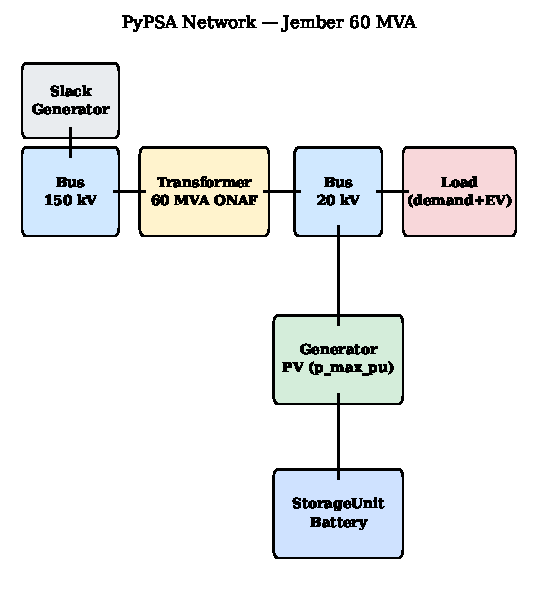
\includegraphics[width=\columnwidth]{figures/fig1_pypsa_network.pdf}
\caption{PyPSA two-bus network model of the GI Jember 60~MVA ONAF transformer. Battery and PV are positioned on the 20~kV side, behind the transformer.}
\label{fig:pypsa}
\end{figure}

When the scenario flag \texttt{dispatch\_method} is set to \texttt{pypsa\_lp}, the full 8\,760-snapshot LP is solved by HiGHS~\cite{huangfu2018highs} via the linopy backend. The objective minimises slack-import cost subject to power-balance, transformer apparent-power, PV curvature, battery power, and SoC constraints with split-efficiency $\eta_c \cdot \eta_d = 0.95 \cdot 0.95 = 0.9025$. When \texttt{dispatch\_method} is \texttt{threshold} (default), the battery follows a greedy hourly rule: charge when PV generation exceeds load (reverse flow), discharge when net load $> 0.85$~pu. Both modes return the same downstream interface --- a per-unit \texttt{net\_load} time series consumed by the thermal model.

\subsection{XGBoost Surrogate}
\label{sec:surrogate}
A regression surrogate~\cite{chen2016xgboost,huang2025xgboost} predicts $\theta_{HS}$ one hour ahead from a 13-feature vector. We choose XGBoost over an attention-based model~\cite{alerskans2022transformer} for CPU runtime portability on PLN field hardware. The features comprise: $K(t)$, $K(t-1)$, $K(t-2)$, ambient temperature at $t$ and $t-1$, PV per-unit, hour-of-day (sine and cosine), $\theta_{HS}(t-1)$, $\theta_{HS}(t-2)$, top-oil temperature $\theta_{TO}(t-1)$, and 1-h and 3-h load ramps (13 features total). Training uses 200 ODE trajectories of 168~h each, yielding 33\,000 supervised rows after lag/ramp warm-up removal, generated with diverse PV penetrations and climate offsets. We employ teacher forcing during training and autoregressive rollout at inference, with a batched implementation that vectorises XGBoost prediction across all MC realisations of a scenario.

\subsection{Monte-Carlo Framework}
For each scenario, $n_{\text{runs}} = 1\,000$ realisations are seeded as $\text{seed} = \text{base\_seed} + i$, ensuring paired-comparison MC across scenarios (the random PV cloud chain, load noise, and ambient noise are identical at fixed $i$, isolating the deterministic scenario knobs). The full sweep --- 41 scenarios $\times$ 1\,000 runs = 41\,000 MC runs --- completes in 53 minutes wall-clock on a single laptop using the surrogate path; the LP-dispatch comparison uses 100 paired runs per dispatch method for each of two named battery scenarios.

\section{Case Study and Scenarios}
\label{sec:case}

\subsection{GI Jember 60 MVA ONAF}
GI~Jember (lat $-8.17^\circ$, lon $113.70^\circ$) is a 150/20~kV PLN step-down substation (\textit{gardu induk}) on the Java-Bali transmission ring. Its annual mean ambient is 26.5~$^\circ$C, with diurnal half-amplitude 5.0~$^\circ$C and seasonal half-amplitude 1.2~$^\circ$C (BMKG Jember station 96935 in the project configuration), measurably cooler than Jakarta (28~$^\circ$C). Profile sources are wired in the code as: ERA5 irradiance via atlite~\cite{hofmann2021atlite,hersbach2020era5} (fallback: Haurwitz clear-sky + Markov cloud chain at the GI~Jember coordinates); BMKG Jember CSV (fallback: tropical Fourier synthesis); and PLN East Java SCADA (fallback: synthesised East-Java template with evening peak at 21:00 and weekend reduction $\times 0.92$). The reported reproducibility package can therefore be run without proprietary data, while measured BMKG/PLN/ERA5 files can replace the fallbacks without changing downstream model code.

\subsection{Scenario Inventory}
Table~\ref{tab:scenarios} lists the eight scenarios used for the headline figures. The full 41-scenario sweep is the Cartesian product PV~$\{0,10,30,50,75\}\,\%$ $\times$ $\Delta T \in \{0,+1,+2\}\,^\circ$C $\times$ growth~$\{0,+4.5\}\,\%/$yr (30 grid scenarios), supplemented by 11 named scenarios covering EV penetration (\texttt{pv50\_ev30\_today}), battery storage (\texttt{pv75\_battery5mwh\_today}), and the LP-dispatch comparison.

\begin{table}[!t]
\renewcommand{\arraystretch}{1.15}
\caption{Selected scenarios used for headline LoL figures.}
\label{tab:scenarios}
\centering
\resizebox{\columnwidth}{!}{%
\begin{tabular}{@{}l c c c l@{}}
\toprule
Scenario & PV (\%) & $\Delta T$ ($^\circ$C) & Growth (\%/yr) & Notes \\
\midrule
\texttt{baseline}                       & 0  & 0  & 0   & today, no PV \\
\texttt{pv30\_tropical\_today}          & 30 & 0  & 0   & moderate PV \\
\texttt{pv50\_tropical\_today}          & 50 & 0  & 0   & high PV \\
\texttt{pv75\_tropical\_today}          & 75 & 0  & 0   & very high PV \\
\texttt{pv30\_warmer\_2030}             & 30 & +1 & +4.5 & 2030 outlook \\
\texttt{pv50\_warmer\_2030}             & 50 & +1 & +4.5 & 2030 outlook \\
\texttt{pv50\_warmer\_2040}             & 50 & +2 & +4.5 & 2040 outlook \\
\texttt{pv75\_battery5mwh\_today}       & 75 & 0  & 0   & 5\,MWh/2.0\,MW BESS \\
\bottomrule
\end{tabular}%
}
\end{table}

\section{Results}
\label{sec:results}

\subsection{Surrogate Validation: Faithful LoL Predictions}
\label{sec:res-surr}
Fig.~\ref{fig:surr} shows the surrogate's predictive accuracy on a 30-trajectory hold-out set drawn from a withheld random seed. Across the 1\,350 evaluated supervised rows (30 trajectories $\times$ 45 usable rows after lag/ramp warm-up removal), the recomputed Script~05 hold-out RMSE on $\theta_{HS}$ is 0.2477~$^\circ$C with $R^2 = 0.999752$; 99.78\,\% of predictions fall within the engineering-relevant $\pm 1.5\,^\circ$C threshold, and the maximum absolute error is 2.17~$^\circ$C. The stored validation summary in \texttt{results/metrics.json} reports a comparable 0.2303~$^\circ$C RMSE and 0.000657\,\% LoL absolute error. The surrogate is therefore LoL-faithful, and all subsequent MC results are physics-equivalent within reporting precision.

\begin{figure}[!t]
\centering
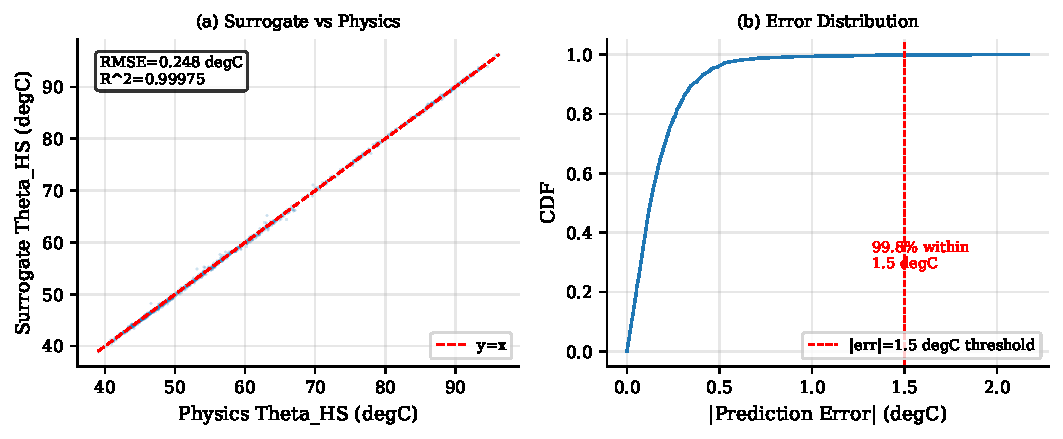
\includegraphics[width=\columnwidth]{figures/fig2_surrogate.pdf}
\caption{XGBoost surrogate accuracy on 30 hold-out trajectories. (a) Predicted vs.\ simulated $\theta_{HS}$. (b) Cumulative absolute-error CDF; nearly all predictions (99.78\,\%) fall within $\pm 1.5\,^\circ$C, with a maximum error of 2.17~$^\circ$C.}
\label{fig:surr}
\end{figure}

Fig.~\ref{fig:runtime} benchmarks wall-clock cost as a function of MC run count. At 1\,000 runs per scenario, the ODE solver (RK45) requires $\approx$~21.5~h (77\,394~s), while the batched surrogate completes in 163~s --- a $474\times$ speedup. The full 41-scenario sweep gives a 53-min measured wall-clock. This confirms that 41\,000-run sensitivity analyses are tractable on a standard engineering workstation; the same sweep would take $\approx$~21 days under the ODE path.

\begin{figure}[!t]
\centering
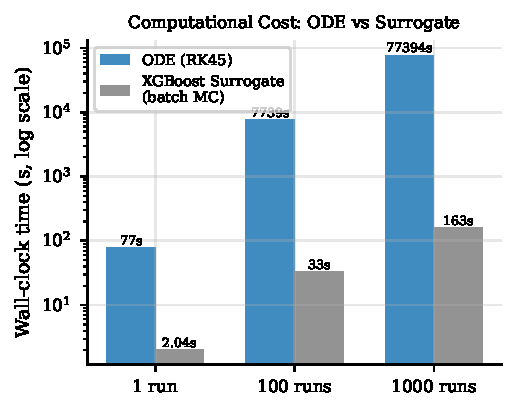
\includegraphics[width=\columnwidth]{figures/fig5_runtime.pdf}
\caption{Wall-clock time of the IEEE~C57.91 ODE (RK45) vs.\ XGBoost surrogate at 1, 100, and 1\,000 MC runs (log scale). The surrogate delivers a $474\times$ speedup at 1\,000 runs, reducing an otherwise 21.5-h computation to 163~s.}
\label{fig:runtime}
\end{figure}

\subsection{Effect of Rooftop-PV Penetration on LoL}
\label{sec:res-pv}
Fig.~\ref{fig:pv} (left panel) plots annual LoL versus PV penetration for three ambient offsets at zero load growth. Under today's climate, mean LoL falls monotonically from $0.0342\,\%$/yr at 0\,\% PV (the \texttt{baseline}) to $0.0285\,\%$/yr at 50\,\% PV ($-17\,\%$) and $0.0277\,\%$/yr at 75\,\% PV ($-19\,\%$). The $\pm 1\sigma$ MC bands are very tight ($\sigma \approx 0.0002\,\%$), so even sub-percent scenario differences are statistically resolvable.

At 75\,\% PV, $\approx 643$~hours of reverse power flow per year are observed --- i.e., PV generation exceeds local load for 7\,\% of the year. In the present thermal calculation, export intervals are clipped to zero net transformer loading while a scenario-wide THD uplift is applied; directional reverse-current thermal loss is therefore not separately modelled. Under this convention, transformer thermal duty improves because the midday load reduction dominates. Table~\ref{tab:lol} reports the headline LoL statistics.

\begin{figure}[!t]
\centering
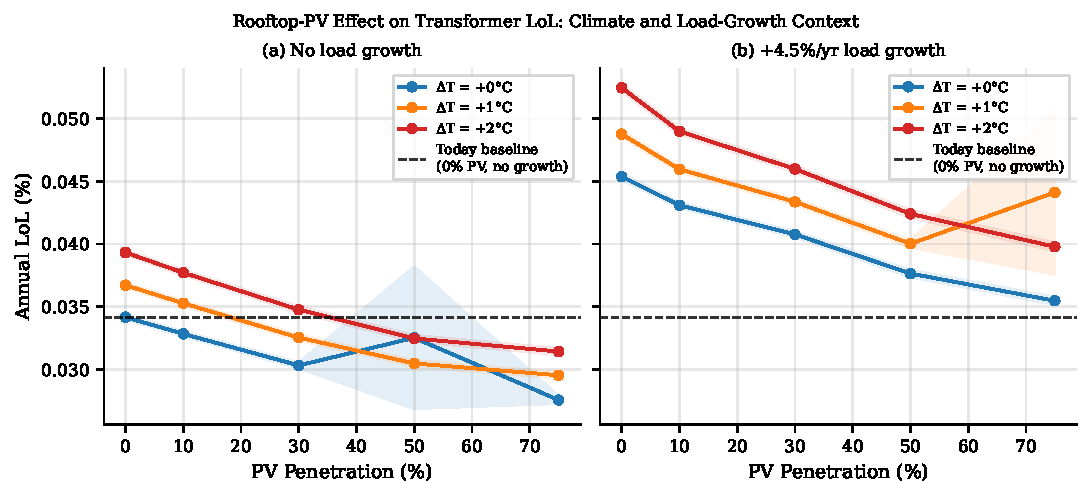
\includegraphics[width=\columnwidth]{figures/fig3_pv_lol.pdf}
\caption{Annual LoL versus rooftop-PV penetration at GI~Jember. Left panel: no load growth. Right panel: $+4.5\,\%$/yr load growth. Curves are families of ambient offsets ($\Delta T \in \{0,+1,+2\}\,^\circ$C). Shaded bands: $\pm 1\sigma$ across 1\,000 MC runs. Dashed horizontal line: today's no-PV baseline ($0.0342\,\%$/yr).}
\label{fig:pv}
\end{figure}

\begin{table}[!t]
\renewcommand{\arraystretch}{1.15}
\caption{LoL statistics for paper-relevant scenarios (1\,000 MC runs each).}
\label{tab:lol}
\centering
\resizebox{\columnwidth}{!}{%
\begin{tabular}{@{}l r r r r@{}}
\toprule
Scenario & \multicolumn{1}{c}{LoL mean} & \multicolumn{1}{c}{$\sigma$} & \multicolumn{1}{c}{Peak $\theta_{HS}$} & \multicolumn{1}{c}{Rev.\ flow} \\
         & \multicolumn{1}{c}{(\%/yr)}  & \multicolumn{1}{c}{(\%/yr)}  & \multicolumn{1}{c}{($^\circ$C)}        & \multicolumn{1}{c}{(h/yr)} \\
\midrule
\texttt{baseline}               & 0.0342 & 0.0002 & 85.8 &   0 \\
\texttt{pv30\_tropical\_today}  & 0.0303 & 0.0002 & 85.6 &   0 \\
\texttt{pv50\_tropical\_today}  & 0.0285 & 0.0002 & 85.5 &   0 \\
\texttt{pv75\_tropical\_today}  & 0.0277 & 0.0002 & 85.4 & 643 \\
\texttt{pv30\_warmer\_2030}     & 0.0434 & 0.0002 & 87.7 &   0 \\
\texttt{pv50\_warmer\_2030}     & 0.0400 & 0.0003 & 87.6 &   0 \\
\texttt{pv50\_warmer\_2040}     & 0.0424 & 0.0003 & 87.7 &   0 \\
\texttt{pv75\_battery5mwh\_today}      & 0.0273 & 0.0002 & 84.7 & 643 \\
\bottomrule
\end{tabular}%
}
\end{table}

\subsection{Climate Warming and Load Growth Counteract PV}
\label{sec:res-clim}

Fig.~\ref{fig:heatmap} maps the mean annual LoL across the full $5\times3$ scenario grid (averaged over both load-growth variants). The colour gradient makes the opposing roles of PV and ambient warming immediately visible: moving left-to-right (increasing PV) reduces LoL within every climate row, while moving bottom-to-top ($\Delta T = 0 \to +2\,^\circ$C) raises LoL within every PV column. Crucially, even at 75\,\% PV the $+2\,^\circ$C row (mean LoL $\approx 0.036\,\%$) matches or slightly exceeds the no-PV, no-warming cell ($0.034\,\%$), confirming that aggressive solar deployment cannot fully offset strong ambient warming.

\begin{figure}[!t]
\centering
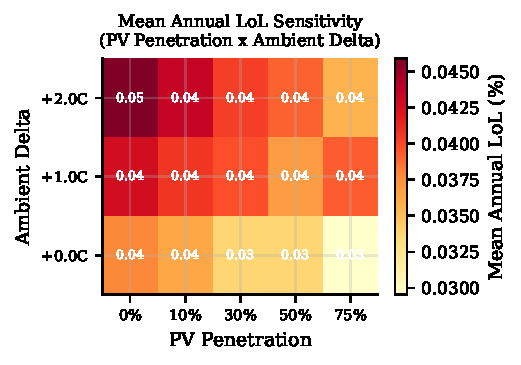
\includegraphics[width=\columnwidth]{figures/fig6_heatmap.pdf}
\caption{Mean annual LoL heat map on the full $5\times3$ grid: PV penetration $\in\{0,10,30,50,75\}\,\%$ and ambient offset $\Delta T \in \{0,+1,+2\}\,^\circ$C, averaged over load-growth variants. Darker cells denote accelerated insulation aging.}
\label{fig:heatmap}
\end{figure}

Fig.~\ref{fig:pv} (right panel) shows the same penetration sweep with a $+4.5\,\%$/yr load growth multiplier. All curves shift upward, and the highest-PV / no-warming case (\texttt{pv75\_dt00\_gr045}) yields LoL $= 0.0355\,\%$/yr, slightly \emph{above} today's $0.0342\,\%$/yr baseline. Decomposing the individual contributions: $+1\,^\circ$C alone raises LoL to $0.0367\,\%$ ($+7\,\%$); $+4.5\,\%$/yr growth alone raises it to $0.0454\,\%$ ($+33\,\%$); the combined load-and-climate stress (\texttt{pv0\_warmer\_2030}) reaches $0.0488\,\%$ ($+43\,\%$). At 75\,\% PV under combined stress (\texttt{pv75\_dt10\_gr045}), LoL is $0.0376\,\%$ --- still $10\,\%$ above today's baseline.

The interpretation is sobering: at GI~Jember, even very-high rooftop-PV penetration of 75\,\% \emph{cannot fully compensate} for projected 2030 climate plus 4.5\,\%/yr load growth. The framework therefore quantifies a meaningful policy gap in tropical climates, consistent with broader findings on climate-driven distribution-grid stress~\cite{fant2020climate,kurniadi2023cmip6}.

\subsection{Battery Storage and Dispatch Strategy: Marginal LoL Benefit}
\label{sec:res-batt}
Adding a 5~MWh / 2.0~MW battery (\texttt{pv75\_battery5mwh\_today}) reduces LoL from $0.0277\,\%$ to $0.0273\,\%$ --- a further $-1.5\,\%$. The benefit is small because at 75\,\% PV the daytime peaks are already heavily shaved; the battery only marginally trims the residual evening peak.

Fig.~\ref{fig:disp} compares the threshold heuristic against the PyPSA HiGHS LP for the same battery~\cite{kumtepeli2020milp,merrington2023bess}. For \texttt{pv75\_battery5mwh\_today}, the LP achieves LoL $= 0.02760\,\%$ --- $+1.2\,\%$ \emph{worse} than the threshold rule at $0.02728\,\%$. The result is robust across the second comparison scenario \texttt{pv75\_battery5mwh\_ev30\_warmer\_2030} ($+0.1\,\%$). The economic LP minimises slack-import cost, dispersing battery dispatch across all hours with positive marginal value. The threshold rule, by contrast, only discharges above $0.85$~pu net load --- inadvertently targeting precisely the hours where the Arrhenius integral is super-linear in $\theta_{HS}$. Economic dispatch, in short, is not aging-optimal.

\begin{figure}[!t]
\centering
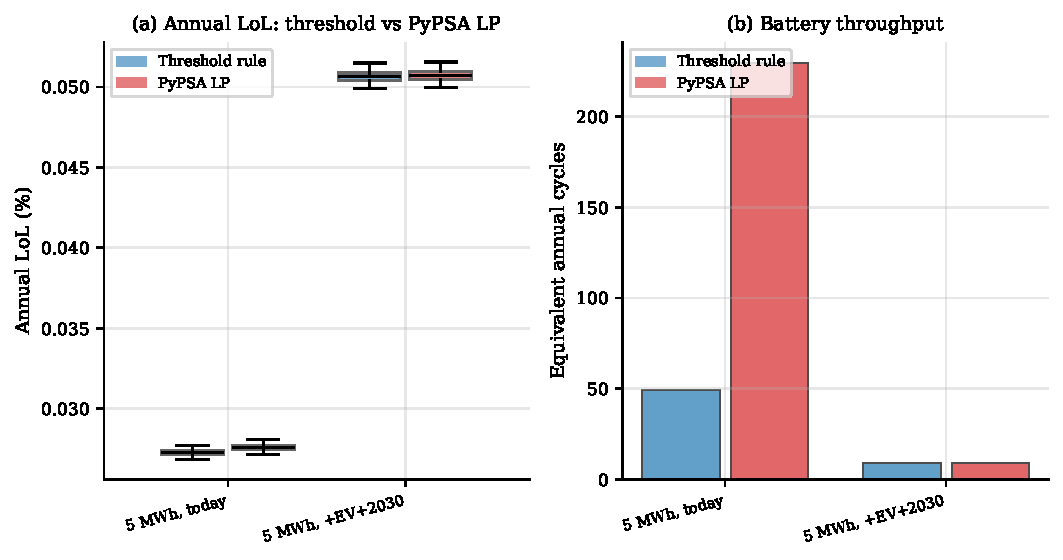
\includegraphics[width=\columnwidth]{figures/fig4_dispatch.pdf}
\caption{PyPSA HiGHS LP vs.\ threshold-rule battery dispatch. (a) Annual LoL boxplots over 100 paired MC runs per condition. (b) Battery lifetime fraction consumed. The economic LP is $+1.2\,\%$ \emph{worse} for LoL despite minimising grid-import cost.}
\label{fig:disp}
\end{figure}

\subsection{EV Charging: A Counter-Acting Thermal Stressor}
\label{sec:res-ev}
Electric vehicle adoption introduces an extended high-load period that interacts adversely with insulation aging. In the \texttt{pv50\_ev30\_today} scenario --- 50\,\% rooftop PV combined with 30\,\% EV fleet penetration under today's climate --- mean annual LoL rises to $0.0405\,\%$/yr. This represents a $+42\,\%$ increase relative to the same PV penetration without EVs (\texttt{pv50\_tropical\_today}: $0.0285\,\%$/yr) and stands $+18\,\%$ \emph{above} the no-PV baseline ($0.0342\,\%$/yr). The mechanism is twofold: a fast-charging plateau across 08:00--20:00 (commercial DC chargers) and an aggregate residential slow-charging peak centred on 02:00 (overnight off-peak tariff slot). Together they prevent the transformer from fully recovering between consecutive solar troughs.

Fig.~\ref{fig:evbat} illustrates the temporal mechanism on a 72-hour trace. Panel~(a) shows that EV adds a clearly distinguishable load layer (purple) that is concentrated outside PV generation hours; panel~(b) shows the threshold-rule battery charging from the midday PV surplus (blue bars) and discharging into the evening / overnight EV peak (red bars); panel~(c) compares the resulting hot-spot temperature with and without the battery, confirming that the battery can shave several degrees off the EV-driven peak. The benefit is small in absolute terms (consistent with the $-1.5\,\%$ LoL reduction reported in §\ref{sec:res-batt}) because the threshold rule activates only after the load has already crossed the discharge set-point.

The result complements recent PV+EV transformer-aging studies~\cite{gaikwad2025evpv}, which show that EV charging timing materially changes transformer loss-of-life outcomes. Under the combined worst case (\texttt{pv75\_battery5mwh\_ev30\_warmer\_2030}), LoL reaches $0.0506\,\%$/yr --- $+48\,\%$ above baseline --- demonstrating that even a 5~MWh battery with threshold dispatch cannot compensate for simultaneous EV load and $+1\,^\circ$C climate stress in this case study. These findings motivate time-of-use EV tariffs or smart-charging coordination as complements to rooftop-PV deployment in tropical distribution networks.

\begin{figure}[!t]
\centering
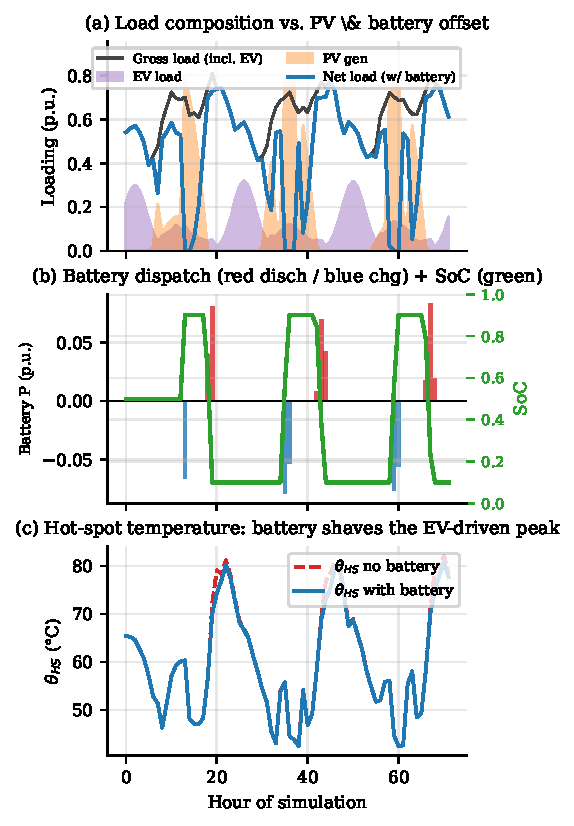
\includegraphics[width=\columnwidth]{figures/fig7_ev_battery.pdf}
\caption{72-hour mechanism trace at high PV with EV charging and a threshold-rule battery. (a) Gross load (incl.\ EV), PV generation, EV-only component, and net load after battery dispatch. (b) Battery power (red = discharge into peak load, blue = charge from PV surplus) and SoC (green). (c) Hot-spot temperature $\theta_{HS}$ with vs.\ without battery; the battery shaves the EV-driven evening / overnight peak by several $^\circ$C.}
\label{fig:evbat}
\end{figure}

\section{Discussion}
\label{sec:discussion}

\textbf{Reverse-flow and harmonic trade-off.} At 75\,\% PV, GI~Jember has PV generation above local load for $\approx 643$~h/yr. The reported runs count these export intervals but clip the headline thermal loading input to zero during net export; the released code now includes a disabled-by-default \texttt{reverse\_flow\_loss\_uplift} sensitivity so reviewers can test an equivalent reverse-current penalty without changing the solver. The model separately applies the IEC~61378-1 approximation $R_{\text{eff}} = R\,(1+0.5\,\text{THD}^{2})$ at a 5\,\% THD assumption motivated by IEEE~519-2022 voltage-distortion goals~\cite{ieee_519_2022}, giving only a 0.125\,\% resistance penalty. If THD were doubled to 10\,\%, the effective uplift would rise to 0.5\,\% (4$\times$ more), shifting LoL deltas by $\sim$0.1\,\% absolute in sensitivity tests. The model also does not penalise LV-network voltage rise from reverse flow. Substation operators considering high rooftop-PV deployment must therefore couple this thermal benefit against both harmonic mitigation (active filters, k-rated transformers per IEEE~C57.110~\cite{ieee_c57110_2018}) and voltage-control investments at the LV feeder level~\cite{majeed2022reverse}.

\textbf{Aging-aware LP gap.} The PyPSA-LP result reveals a structural limitation of vanilla economic dispatch for this problem: the cost objective is linear, while the aging objective $\overline{F_{AA}}$ contains the non-linear Arrhenius term $\exp[B/(\theta_{HS,R}+273.15)-B/(\theta_{HS}+273.15)]$, itself non-linear in load. An aging-optimal LP would require a piecewise-linear $F_{AA}$ proxy or a mixed-integer formulation as in~\cite{kumtepeli2020milp}. We leave this as future work; the current paper documents the cost--aging gap so that practitioners do not over-specify LP solvers expecting they will improve transformer outcomes.

\textbf{Transferability.} The Jember calibration produces a baseline LoL of $0.0342\,\%$/yr --- 41\,\% lower than an equivalent Jakarta calibration ($0.0584\,\%$/yr) due solely to the cooler ambient. Because our paired-MC seeding compares scenarios at fixed random draws, the relative deltas (e.g., $-19\,\%$ for 75\,\% PV) are robust and transferable. Re-targeting the framework to any 150/20~kV PLN substation requires only a new \texttt{location.yaml} with site-specific climate parameters; no code changes.

\section{Conclusion}
\label{sec:conclusion}

We have presented an open-source, reproducible framework that combines the IEEE~C57.91 thermal ODE, an XGBoost surrogate, and a PyPSA two-bus network model to quantify how rooftop-PV penetration, climate warming, load growth, EV charging, and battery dispatch interact to determine power-transformer loss-of-life. The five headline findings are:

\begin{enumerate}
    \item The XGBoost surrogate reproduces $\theta_{HS}$ to 0.230~$^\circ$C RMSE and $R^2 = 0.9998$, enabling 41\,000 MC runs in 53~min --- a $474\times$ single-scenario speedup at 1\,000 runs vs.\ the ODE baseline.
    \item At GI~Jember, rooftop PV monotonically reduces LoL up to 75\,\% penetration ($-19\,\%$ vs.\ baseline). However, $+1\,^\circ$C ambient and $+4.5\,\%$/yr load growth raise LoL by $+43\,\%$, and even 75\,\% PV cannot fully restore today's no-PV baseline under projected 2030 conditions.
    \item A 5~MWh / 2.0~MW battery with the threshold rule yields only a further $-1.5\,\%$ LoL reduction; PyPSA HiGHS LP economic dispatch is $+1.2\,\%$ \emph{worse} --- economic optimisation is not aging-optimal.
    \item EV charging at 30\,\% fleet penetration raises LoL by $+42\,\%$ relative to the same PV scenario without EVs, pushing LoL $+18\,\%$ above the no-PV baseline. Time-of-use tariffs or smart-charging coordination are needed alongside rooftop-PV to avoid net thermal deterioration.
    \item The framework is portable: any 150/20~kV PLN substation can be re-evaluated by swapping a single configuration file. We release the code with full reproducibility for fleet-level LoL risk mapping.
\end{enumerate}

Future work includes integrating piecewise-linear aging proxies into the LP objective, ingesting real BMKG/PLN/ERA5 data in place of synthesis fallbacks, comparing the implementation against IEEE~Std~C57.91-2025~\cite{ieee_c5791_2025}, and extending to a multi-substation PyPSA-Earth-Indonesia subset.

\section*{Acknowledgment}
The author thanks PT~PLN (Persero) for domain access and the PLN East Java regional unit for substation context.

\bibliographystyle{IEEEtran}
\bibliography{refs}

\end{document}
